\subsection{UC3 - Riduzione dimensionale}
\begin{figure}[h]
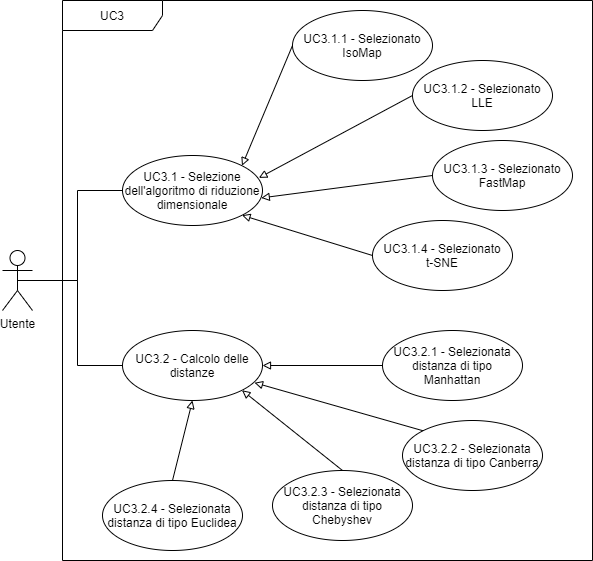
\includegraphics[width=9cm]{section/Images/UC3.png}
\centering
\caption{UC3 - Riduzione dimensionale}
\end{figure}
\begin{itemize}
	\item \textbf{Attore primario}: Utente;
	\item \textbf{Precondizioni}: L'utente ha selezionato le dimensioni da utilizzare [UC2];
	\item \textbf{Postcondizioni}: La scelta viene memorizzata nel sistema e viene resa disponibile una sezione per la personalizzazione dei parametri a seconda del tipo di riduzione dimensionale selezionato [UC4];
	\item \textbf{Scenario principale}: L'utente seleziona un tipo di riduzione dimensionale tra quelli resi disponibili dal sistema.
\end{itemize}